\documentclass[twoside]{book}

% Packages required by doxygen
\usepackage{fixltx2e}
\usepackage{calc}
\usepackage{doxygen}
\usepackage[export]{adjustbox} % also loads graphicx
\usepackage{graphicx}
\usepackage[utf8]{inputenc}
\usepackage{makeidx}
\usepackage{multicol}
\usepackage{multirow}
\PassOptionsToPackage{warn}{textcomp}
\usepackage{textcomp}
\usepackage[nointegrals]{wasysym}
\usepackage[table]{xcolor}

% Font selection
\usepackage[T1]{fontenc}
\usepackage[scaled=.90]{helvet}
\usepackage{courier}
\usepackage{amssymb}
\usepackage{sectsty}
\renewcommand{\familydefault}{\sfdefault}
\allsectionsfont{%
  \fontseries{bc}\selectfont%
  \color{darkgray}%
}
\renewcommand{\DoxyLabelFont}{%
  \fontseries{bc}\selectfont%
  \color{darkgray}%
}
\newcommand{\+}{\discretionary{\mbox{\scriptsize$\hookleftarrow$}}{}{}}

% Page & text layout
\usepackage{geometry}
\geometry{%
  a4paper,%
  top=2.5cm,%
  bottom=2.5cm,%
  left=2.5cm,%
  right=2.5cm%
}
\tolerance=750
\hfuzz=15pt
\hbadness=750
\setlength{\emergencystretch}{15pt}
\setlength{\parindent}{0cm}
\setlength{\parskip}{3ex plus 2ex minus 2ex}
\makeatletter
\renewcommand{\paragraph}{%
  \@startsection{paragraph}{4}{0ex}{-1.0ex}{1.0ex}{%
    \normalfont\normalsize\bfseries\SS@parafont%
  }%
}
\renewcommand{\subparagraph}{%
  \@startsection{subparagraph}{5}{0ex}{-1.0ex}{1.0ex}{%
    \normalfont\normalsize\bfseries\SS@subparafont%
  }%
}
\makeatother

% Headers & footers
\usepackage{fancyhdr}
\pagestyle{fancyplain}
\fancyhead[LE]{\fancyplain{}{\bfseries\thepage}}
\fancyhead[CE]{\fancyplain{}{}}
\fancyhead[RE]{\fancyplain{}{\bfseries\leftmark}}
\fancyhead[LO]{\fancyplain{}{\bfseries\rightmark}}
\fancyhead[CO]{\fancyplain{}{}}
\fancyhead[RO]{\fancyplain{}{\bfseries\thepage}}
\fancyfoot[LE]{\fancyplain{}{}}
\fancyfoot[CE]{\fancyplain{}{}}
\fancyfoot[RE]{\fancyplain{}{\bfseries\scriptsize Generated by Doxygen }}
\fancyfoot[LO]{\fancyplain{}{\bfseries\scriptsize Generated by Doxygen }}
\fancyfoot[CO]{\fancyplain{}{}}
\fancyfoot[RO]{\fancyplain{}{}}
\renewcommand{\footrulewidth}{0.4pt}
\renewcommand{\chaptermark}[1]{%
  \markboth{#1}{}%
}
\renewcommand{\sectionmark}[1]{%
  \markright{\thesection\ #1}%
}

% Indices & bibliography
\usepackage{natbib}
\usepackage[titles]{tocloft}
\setcounter{tocdepth}{3}
\setcounter{secnumdepth}{5}
\makeindex

% Hyperlinks (required, but should be loaded last)
\usepackage{ifpdf}
\ifpdf
  \usepackage[pdftex,pagebackref=true]{hyperref}
\else
  \usepackage[ps2pdf,pagebackref=true]{hyperref}
\fi
\hypersetup{%
  colorlinks=true,%
  linkcolor=blue,%
  citecolor=blue,%
  unicode%
}

% Custom commands
\newcommand{\clearemptydoublepage}{%
  \newpage{\pagestyle{empty}\cleardoublepage}%
}

\usepackage{caption}
\captionsetup{labelsep=space,justification=centering,font={bf},singlelinecheck=off,skip=4pt,position=top}

%===== C O N T E N T S =====

\begin{document}

% Titlepage & ToC
\hypersetup{pageanchor=false,
             bookmarksnumbered=true,
             pdfencoding=unicode
            }
\pagenumbering{alph}
\begin{titlepage}
\vspace*{7cm}
\begin{center}%
{\Large P\+Eter }\\
\vspace*{1cm}
{\large Generated by Doxygen 1.8.13}\\
\end{center}
\end{titlepage}
\clearemptydoublepage
\pagenumbering{roman}
\tableofcontents
\clearemptydoublepage
\pagenumbering{arabic}
\hypersetup{pageanchor=true}

%--- Begin generated contents ---
\chapter{P\+Eter}
\label{index}\hypertarget{index}{}\hypertarget{index_Introduction}{}\section{Introduction}\label{index_Introduction}
\hypertarget{index_hdrs}{}\subsection{hdrs}\label{index_hdrs}
This library helps you change Portable Executables. Right now you can just alter the export and import headers and the section table. Of Cause you can change the raw MZ and NT Headers as well. This is how it works\+: 
\begin{DoxyCode}
hdrs h;
hdrs\_init(&h, file);
printf(\textcolor{stringliteral}{"PE files entry point (RVA): 0x%x\(\backslash\)n"},
       hdrs\_get\_address\_of\_entry\_point(&h));
hdrs\_destroy(&h);
\end{DoxyCode}
 This exeample will print the value of the Address\+Of\+Entry\+Point field. You can get almost all other header values by using functions starting with the hdrs\+\_\+ prefix. They are build up like this\+: hdrs\+\_\+$<$set/get$>$\+\_\+field\+\_\+name(hdrs $\ast$hdrs\+Object) if set was choosen then you give it a second parameter which contains the value you want to set. \hypertarget{index_imports}{}\subsection{exports sections}\label{index_imports}
The functions for maipulating imports, exports and sections are documented. In their header files (\hyperlink{sections_8h}{sections.\+h}, \hyperlink{imports_8h}{imports.\+h}, \hyperlink{exports_8h}{exports.\+h}). They don\textquotesingle{}t need an init() function to be called. You can just use them with a pointer to the raw file image you want to work with. 
\chapter{File Index}
\section{File List}
Here is a list of all documented files with brief descriptions\+:\begin{DoxyCompactList}
\item\contentsline{section}{/home/x/git-\/repos/\+P\+Eter/src/\hyperlink{exports_8h}{exports.\+h} \\*These functions can be used to get information from a PE files export header }{\pageref{exports_8h}}{}
\item\contentsline{section}{/home/x/git-\/repos/\+P\+Eter/src/\hyperlink{imports_8h}{imports.\+h} \\*These functions give you information about the import table }{\pageref{imports_8h}}{}
\item\contentsline{section}{/home/x/git-\/repos/\+P\+Eter/src/\hyperlink{peter_8h}{peter.\+h} \\*This file is the file you can actually include for using the library. It does nothing but including other header files }{\pageref{peter_8h}}{}
\item\contentsline{section}{/home/x/git-\/repos/\+P\+Eter/src/\hyperlink{sections_8h}{sections.\+h} \\*This file contains functions for getting information concerning the section headers (e.\+g. \hyperlink{sections_8h_a4846d5524cb1771349480ba3fa53aa5b}{sections\+\_\+by\+\_\+name\+\_\+is\+\_\+writable()} informs you wether the writable flag in a section header is set). An other type of function changes the values within the section headers (set functions like \hyperlink{sections_8h_af3c1453de2d6655bf83c8373237cbf67}{sections\+\_\+by\+\_\+name\+\_\+set\+\_\+name()} ) or may even add a new one. The functions which convert e.\+g. pointers to rva values where placed in this header too, because they need information from the section headers to calculate their return values }{\pageref{sections_8h}}{}
\end{DoxyCompactList}

\chapter{File Documentation}
\hypertarget{exports_8h}{}\section{/home/x/git-\/repos/\+P\+Eter/src/exports.h File Reference}
\label{exports_8h}\index{/home/x/git-\/repos/\+P\+Eter/src/exports.\+h@{/home/x/git-\/repos/\+P\+Eter/src/exports.\+h}}


These functions can be used to get information from a PE files export header.  


This graph shows which files directly or indirectly include this file\+:
\nopagebreak
\begin{figure}[H]
\begin{center}
\leavevmode
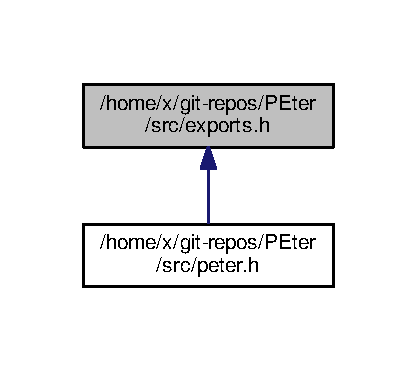
\includegraphics[width=200pt]{exports_8h__dep__incl}
\end{center}
\end{figure}
\subsection*{Functions}
\begin{DoxyCompactItemize}
\item 
uint16\+\_\+t \hyperlink{exports_8h_a09859e90782da27c2402faa733c6c208}{exports\+\_\+get\+\_\+ordinal\+\_\+by\+\_\+name} (void $\ast$image, const char $\ast$name)
\begin{DoxyCompactList}\small\item\em returns the ordinal for the function you name \end{DoxyCompactList}\item 
void $\ast$ \hyperlink{exports_8h_a4490ee501168af2361054f4679b318ab}{exports\+\_\+get\+\_\+function\+\_\+by\+\_\+name} (void $\ast$image, const char $\ast$name)
\begin{DoxyCompactList}\small\item\em returns a functions address \end{DoxyCompactList}\item 
char $\ast$ \hyperlink{exports_8h_af4c32bfeafff566f20334782e38a0397}{exports\+\_\+get\+\_\+name\+\_\+by\+\_\+index} (void $\ast$image, const uint32\+\_\+t idx)
\begin{DoxyCompactList}\small\item\em returns the first function name in the export headerif idx = 0, the second if idx = 1 and so on \end{DoxyCompactList}\item 
void $\ast$ \hyperlink{exports_8h_adda1f24d002772947aa4a4daf885e489}{exports\+\_\+get\+\_\+function\+\_\+by\+\_\+ordinal} (void $\ast$image, uint32\+\_\+t ord)
\begin{DoxyCompactList}\small\item\em you give it an ordinal and you get a pointer to a function \end{DoxyCompactList}\end{DoxyCompactItemize}


\subsection{Detailed Description}
These functions can be used to get information from a PE files export header. 



\subsection{Function Documentation}
\mbox{\Hypertarget{exports_8h_a4490ee501168af2361054f4679b318ab}\label{exports_8h_a4490ee501168af2361054f4679b318ab}} 
\index{exports.\+h@{exports.\+h}!exports\+\_\+get\+\_\+function\+\_\+by\+\_\+name@{exports\+\_\+get\+\_\+function\+\_\+by\+\_\+name}}
\index{exports\+\_\+get\+\_\+function\+\_\+by\+\_\+name@{exports\+\_\+get\+\_\+function\+\_\+by\+\_\+name}!exports.\+h@{exports.\+h}}
\subsubsection{\texorpdfstring{exports\+\_\+get\+\_\+function\+\_\+by\+\_\+name()}{exports\_get\_function\_by\_name()}}
{\footnotesize\ttfamily void$\ast$ exports\+\_\+get\+\_\+function\+\_\+by\+\_\+name (\begin{DoxyParamCaption}\item[{void $\ast$}]{image,  }\item[{const char $\ast$}]{name }\end{DoxyParamCaption})}



returns a functions address 


\begin{DoxyParams}{Parameters}
{\em image} & is a pointer to the pe image you want to analyze \\
\hline
{\em name} & is a pointer on the name of the A\+PI function you want the address of \\
\hline
\end{DoxyParams}
\mbox{\Hypertarget{exports_8h_adda1f24d002772947aa4a4daf885e489}\label{exports_8h_adda1f24d002772947aa4a4daf885e489}} 
\index{exports.\+h@{exports.\+h}!exports\+\_\+get\+\_\+function\+\_\+by\+\_\+ordinal@{exports\+\_\+get\+\_\+function\+\_\+by\+\_\+ordinal}}
\index{exports\+\_\+get\+\_\+function\+\_\+by\+\_\+ordinal@{exports\+\_\+get\+\_\+function\+\_\+by\+\_\+ordinal}!exports.\+h@{exports.\+h}}
\subsubsection{\texorpdfstring{exports\+\_\+get\+\_\+function\+\_\+by\+\_\+ordinal()}{exports\_get\_function\_by\_ordinal()}}
{\footnotesize\ttfamily void$\ast$ exports\+\_\+get\+\_\+function\+\_\+by\+\_\+ordinal (\begin{DoxyParamCaption}\item[{void $\ast$}]{image,  }\item[{uint32\+\_\+t}]{ord }\end{DoxyParamCaption})}



you give it an ordinal and you get a pointer to a function 


\begin{DoxyParams}{Parameters}
{\em image} & $<$-- like above \\
\hline
{\em ord} & should be one of the values you can find in the odinal list of the P\+Es export table. \\
\hline
\end{DoxyParams}
\mbox{\Hypertarget{exports_8h_af4c32bfeafff566f20334782e38a0397}\label{exports_8h_af4c32bfeafff566f20334782e38a0397}} 
\index{exports.\+h@{exports.\+h}!exports\+\_\+get\+\_\+name\+\_\+by\+\_\+index@{exports\+\_\+get\+\_\+name\+\_\+by\+\_\+index}}
\index{exports\+\_\+get\+\_\+name\+\_\+by\+\_\+index@{exports\+\_\+get\+\_\+name\+\_\+by\+\_\+index}!exports.\+h@{exports.\+h}}
\subsubsection{\texorpdfstring{exports\+\_\+get\+\_\+name\+\_\+by\+\_\+index()}{exports\_get\_name\_by\_index()}}
{\footnotesize\ttfamily char$\ast$ exports\+\_\+get\+\_\+name\+\_\+by\+\_\+index (\begin{DoxyParamCaption}\item[{void $\ast$}]{image,  }\item[{const uint32\+\_\+t}]{idx }\end{DoxyParamCaption})}



returns the first function name in the export headerif idx = 0, the second if idx = 1 and so on 


\begin{DoxyParams}{Parameters}
{\em image} & is a pointer on the pe image \\
\hline
{\em idx} & is 0 for the first name and so on... (like an array index) \\
\hline
\end{DoxyParams}
\mbox{\Hypertarget{exports_8h_a09859e90782da27c2402faa733c6c208}\label{exports_8h_a09859e90782da27c2402faa733c6c208}} 
\index{exports.\+h@{exports.\+h}!exports\+\_\+get\+\_\+ordinal\+\_\+by\+\_\+name@{exports\+\_\+get\+\_\+ordinal\+\_\+by\+\_\+name}}
\index{exports\+\_\+get\+\_\+ordinal\+\_\+by\+\_\+name@{exports\+\_\+get\+\_\+ordinal\+\_\+by\+\_\+name}!exports.\+h@{exports.\+h}}
\subsubsection{\texorpdfstring{exports\+\_\+get\+\_\+ordinal\+\_\+by\+\_\+name()}{exports\_get\_ordinal\_by\_name()}}
{\footnotesize\ttfamily uint16\+\_\+t exports\+\_\+get\+\_\+ordinal\+\_\+by\+\_\+name (\begin{DoxyParamCaption}\item[{void $\ast$}]{image,  }\item[{const char $\ast$}]{name }\end{DoxyParamCaption})}



returns the ordinal for the function you name 


\begin{DoxyParams}{Parameters}
{\em image} & is a pointer to the first byte of the image you want to analyze \\
\hline
{\em name} & is a pointer on the name of the function you want to get the ordinal of \\
\hline
\end{DoxyParams}

\hypertarget{imports_8h}{}\section{/home/x/git-\/repos/\+P\+Eter/src/imports.h File Reference}
\label{imports_8h}\index{/home/x/git-\/repos/\+P\+Eter/src/imports.\+h@{/home/x/git-\/repos/\+P\+Eter/src/imports.\+h}}


These functions give you information about the import table.  


This graph shows which files directly or indirectly include this file\+:
\nopagebreak
\begin{figure}[H]
\begin{center}
\leavevmode
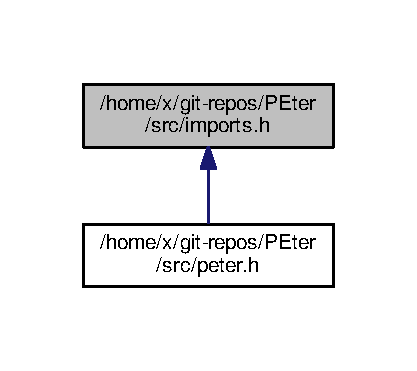
\includegraphics[width=200pt]{imports_8h__dep__incl}
\end{center}
\end{figure}
\subsection*{Functions}
\begin{DoxyCompactItemize}
\item 
I\+M\+A\+G\+E\+\_\+\+I\+M\+P\+O\+R\+T\+\_\+\+D\+E\+S\+C\+R\+I\+P\+T\+OR $\ast$ \hyperlink{imports_8h_a8036faf1c005de380202f58ce21d7d69}{imports\+\_\+by\+\_\+index\+\_\+get\+\_\+import\+\_\+descriptor} (void $\ast$image, int i)
\begin{DoxyCompactList}\small\item\em return the import descriptor with the index i \end{DoxyCompactList}\item 
char $\ast$ \hyperlink{imports_8h_a86884a4f94524df4230d626c416cb861}{imports\+\_\+by\+\_\+index\+\_\+get\+\_\+name} (void $\ast$image, int i)
\begin{DoxyCompactList}\small\item\em returns a char $\ast$pointer on the import descriptors name (the dll name) \end{DoxyCompactList}\item 
int \hyperlink{imports_8h_a97c863ceb042fe8400260af874ab20a5}{imports\+\_\+by\+\_\+name\+\_\+get\+\_\+index} (void $\ast$image, const char $\ast$name)
\begin{DoxyCompactList}\small\item\em returns the import descroptor index that fits the name parameter \end{DoxyCompactList}\item 
int \hyperlink{imports_8h_a46d844dcd94f11ce99b7e158588ac4a9}{imports\+\_\+by\+\_\+name\+\_\+get\+\_\+iname\+\_\+index\+\_\+by\+\_\+name} (void $\ast$image, const char $\ast$dll\+Name, const char $\ast$func\+Name)
\begin{DoxyCompactList}\small\item\em returns the index of the imported fucntion of a dll (that\textquotesingle{}s not an ordinal) \end{DoxyCompactList}\item 
I\+M\+A\+G\+E\+\_\+\+I\+M\+P\+O\+R\+T\+\_\+\+B\+Y\+\_\+\+N\+A\+ME $\ast$ \hyperlink{imports_8h_a9a64f9e3e4b74e10be4770f1f6be8595}{imports\+\_\+by\+\_\+index\+\_\+get\+\_\+iname\+\_\+by\+\_\+index} (void $\ast$image, int idt\+Idx, int int\+Idx)
\begin{DoxyCompactList}\small\item\em you give it two indexes (import descriptor and its import name table) and you get the name of the function these two indexes discribe. That means you will get the first function name of the first imported dll if idt\+Idx and int\+Idx are both == 0. The returned pointer is an I\+M\+A\+G\+E\+\_\+\+I\+M\+P\+O\+R\+T\+\_\+\+B\+Y\+\_\+\+N\+A\+ME struct which is actually a uint8\+\_\+t array but with a word (16bit) value at its start. \end{DoxyCompactList}\item 
void $\ast$ \hyperlink{imports_8h_ab9faff9e489626206a9a65fa6ddbe30e}{imports\+\_\+by\+\_\+index\+\_\+get\+\_\+iaddr\+\_\+thunk\+\_\+by\+\_\+index} (void $\ast$image, int idt\+Idx, int iat\+Idx)
\begin{DoxyCompactList}\small\item\em like \hyperlink{imports_8h_a9a64f9e3e4b74e10be4770f1f6be8595}{imports\+\_\+by\+\_\+index\+\_\+get\+\_\+iname\+\_\+by\+\_\+index()} but doesn\textquotesingle{}t return a name but a pointer on I\+M\+A\+G\+E\+\_\+\+T\+H\+U\+N\+K\+\_\+\+D\+A\+TA if it\textquotesingle{}s a 32bit executable this function will return I\+M\+A\+G\+E\+\_\+\+T\+H\+U\+N\+K\+\_\+\+D\+A\+T\+A32 and if you have 64bit you may use the return value as a pointer on I\+M\+A\+G\+E\+\_\+\+T\+H\+U\+N\+K\+\_\+\+D\+A\+T\+A64 \end{DoxyCompactList}\item 
void \hyperlink{imports_8h_aef79655590df81878c67d7addb032f58}{imports\+\_\+by\+\_\+index\+\_\+set\+\_\+iaddr\+\_\+thunk\+\_\+by\+\_\+index} (void $\ast$image, int idt\+Idx, int iat\+Idx, void $\ast$address)
\begin{DoxyCompactList}\small\item\em Writes an address into the specified field of the import address table. \end{DoxyCompactList}\end{DoxyCompactItemize}


\subsection{Detailed Description}
These functions give you information about the import table. 



\subsection{Function Documentation}
\mbox{\Hypertarget{imports_8h_ab9faff9e489626206a9a65fa6ddbe30e}\label{imports_8h_ab9faff9e489626206a9a65fa6ddbe30e}} 
\index{imports.\+h@{imports.\+h}!imports\+\_\+by\+\_\+index\+\_\+get\+\_\+iaddr\+\_\+thunk\+\_\+by\+\_\+index@{imports\+\_\+by\+\_\+index\+\_\+get\+\_\+iaddr\+\_\+thunk\+\_\+by\+\_\+index}}
\index{imports\+\_\+by\+\_\+index\+\_\+get\+\_\+iaddr\+\_\+thunk\+\_\+by\+\_\+index@{imports\+\_\+by\+\_\+index\+\_\+get\+\_\+iaddr\+\_\+thunk\+\_\+by\+\_\+index}!imports.\+h@{imports.\+h}}
\subsubsection{\texorpdfstring{imports\+\_\+by\+\_\+index\+\_\+get\+\_\+iaddr\+\_\+thunk\+\_\+by\+\_\+index()}{imports\_by\_index\_get\_iaddr\_thunk\_by\_index()}}
{\footnotesize\ttfamily void$\ast$ imports\+\_\+by\+\_\+index\+\_\+get\+\_\+iaddr\+\_\+thunk\+\_\+by\+\_\+index (\begin{DoxyParamCaption}\item[{void $\ast$}]{image,  }\item[{int}]{idt\+Idx,  }\item[{int}]{iat\+Idx }\end{DoxyParamCaption})}



like \hyperlink{imports_8h_a9a64f9e3e4b74e10be4770f1f6be8595}{imports\+\_\+by\+\_\+index\+\_\+get\+\_\+iname\+\_\+by\+\_\+index()} but doesn\textquotesingle{}t return a name but a pointer on I\+M\+A\+G\+E\+\_\+\+T\+H\+U\+N\+K\+\_\+\+D\+A\+TA if it\textquotesingle{}s a 32bit executable this function will return I\+M\+A\+G\+E\+\_\+\+T\+H\+U\+N\+K\+\_\+\+D\+A\+T\+A32 and if you have 64bit you may use the return value as a pointer on I\+M\+A\+G\+E\+\_\+\+T\+H\+U\+N\+K\+\_\+\+D\+A\+T\+A64 


\begin{DoxyParams}{Parameters}
{\em image} & is the PE file \\
\hline
{\em idt\+Idx} & is an import descriptor index \\
\hline
{\em iat\+Idx} & is the address table index \\
\hline
\end{DoxyParams}
\mbox{\Hypertarget{imports_8h_a8036faf1c005de380202f58ce21d7d69}\label{imports_8h_a8036faf1c005de380202f58ce21d7d69}} 
\index{imports.\+h@{imports.\+h}!imports\+\_\+by\+\_\+index\+\_\+get\+\_\+import\+\_\+descriptor@{imports\+\_\+by\+\_\+index\+\_\+get\+\_\+import\+\_\+descriptor}}
\index{imports\+\_\+by\+\_\+index\+\_\+get\+\_\+import\+\_\+descriptor@{imports\+\_\+by\+\_\+index\+\_\+get\+\_\+import\+\_\+descriptor}!imports.\+h@{imports.\+h}}
\subsubsection{\texorpdfstring{imports\+\_\+by\+\_\+index\+\_\+get\+\_\+import\+\_\+descriptor()}{imports\_by\_index\_get\_import\_descriptor()}}
{\footnotesize\ttfamily I\+M\+A\+G\+E\+\_\+\+I\+M\+P\+O\+R\+T\+\_\+\+D\+E\+S\+C\+R\+I\+P\+T\+OR$\ast$ imports\+\_\+by\+\_\+index\+\_\+get\+\_\+import\+\_\+descriptor (\begin{DoxyParamCaption}\item[{void $\ast$}]{image,  }\item[{int}]{idt\+Idx }\end{DoxyParamCaption})}



return the import descriptor with the index i 


\begin{DoxyParams}{Parameters}
{\em image} & points to the image you want to analyze \\
\hline
{\em i} & is 0 if you need the first import descriptor i = 1 for the second and so on \\
\hline
\end{DoxyParams}
\mbox{\Hypertarget{imports_8h_a9a64f9e3e4b74e10be4770f1f6be8595}\label{imports_8h_a9a64f9e3e4b74e10be4770f1f6be8595}} 
\index{imports.\+h@{imports.\+h}!imports\+\_\+by\+\_\+index\+\_\+get\+\_\+iname\+\_\+by\+\_\+index@{imports\+\_\+by\+\_\+index\+\_\+get\+\_\+iname\+\_\+by\+\_\+index}}
\index{imports\+\_\+by\+\_\+index\+\_\+get\+\_\+iname\+\_\+by\+\_\+index@{imports\+\_\+by\+\_\+index\+\_\+get\+\_\+iname\+\_\+by\+\_\+index}!imports.\+h@{imports.\+h}}
\subsubsection{\texorpdfstring{imports\+\_\+by\+\_\+index\+\_\+get\+\_\+iname\+\_\+by\+\_\+index()}{imports\_by\_index\_get\_iname\_by\_index()}}
{\footnotesize\ttfamily I\+M\+A\+G\+E\+\_\+\+I\+M\+P\+O\+R\+T\+\_\+\+B\+Y\+\_\+\+N\+A\+ME$\ast$ imports\+\_\+by\+\_\+index\+\_\+get\+\_\+iname\+\_\+by\+\_\+index (\begin{DoxyParamCaption}\item[{void $\ast$}]{image,  }\item[{int}]{idt\+Idx,  }\item[{int}]{int\+Idx }\end{DoxyParamCaption})}



you give it two indexes (import descriptor and its import name table) and you get the name of the function these two indexes discribe. That means you will get the first function name of the first imported dll if idt\+Idx and int\+Idx are both == 0. The returned pointer is an I\+M\+A\+G\+E\+\_\+\+I\+M\+P\+O\+R\+T\+\_\+\+B\+Y\+\_\+\+N\+A\+ME struct which is actually a uint8\+\_\+t array but with a word (16bit) value at its start. 


\begin{DoxyParams}{Parameters}
{\em image} & points to the PE file \\
\hline
{\em idt\+Idx} & is the import descriptor index (starting at 0 for the first import descriptor) \\
\hline
{\em int\+Idx} & is the name table index (also starting with 0) \\
\hline
\end{DoxyParams}
\mbox{\Hypertarget{imports_8h_a86884a4f94524df4230d626c416cb861}\label{imports_8h_a86884a4f94524df4230d626c416cb861}} 
\index{imports.\+h@{imports.\+h}!imports\+\_\+by\+\_\+index\+\_\+get\+\_\+name@{imports\+\_\+by\+\_\+index\+\_\+get\+\_\+name}}
\index{imports\+\_\+by\+\_\+index\+\_\+get\+\_\+name@{imports\+\_\+by\+\_\+index\+\_\+get\+\_\+name}!imports.\+h@{imports.\+h}}
\subsubsection{\texorpdfstring{imports\+\_\+by\+\_\+index\+\_\+get\+\_\+name()}{imports\_by\_index\_get\_name()}}
{\footnotesize\ttfamily char$\ast$ imports\+\_\+by\+\_\+index\+\_\+get\+\_\+name (\begin{DoxyParamCaption}\item[{void $\ast$}]{image,  }\item[{int}]{idt\+Idx }\end{DoxyParamCaption})}



returns a char $\ast$pointer on the import descriptors name (the dll name) 


\begin{DoxyParams}{Parameters}
{\em image} & points tor the image you want to analyzee \\
\hline
{\em i} & is an index indicating which import disc. you want the name of (starting with 0) \\
\hline
\end{DoxyParams}
\mbox{\Hypertarget{imports_8h_aef79655590df81878c67d7addb032f58}\label{imports_8h_aef79655590df81878c67d7addb032f58}} 
\index{imports.\+h@{imports.\+h}!imports\+\_\+by\+\_\+index\+\_\+set\+\_\+iaddr\+\_\+thunk\+\_\+by\+\_\+index@{imports\+\_\+by\+\_\+index\+\_\+set\+\_\+iaddr\+\_\+thunk\+\_\+by\+\_\+index}}
\index{imports\+\_\+by\+\_\+index\+\_\+set\+\_\+iaddr\+\_\+thunk\+\_\+by\+\_\+index@{imports\+\_\+by\+\_\+index\+\_\+set\+\_\+iaddr\+\_\+thunk\+\_\+by\+\_\+index}!imports.\+h@{imports.\+h}}
\subsubsection{\texorpdfstring{imports\+\_\+by\+\_\+index\+\_\+set\+\_\+iaddr\+\_\+thunk\+\_\+by\+\_\+index()}{imports\_by\_index\_set\_iaddr\_thunk\_by\_index()}}
{\footnotesize\ttfamily void imports\+\_\+by\+\_\+index\+\_\+set\+\_\+iaddr\+\_\+thunk\+\_\+by\+\_\+index (\begin{DoxyParamCaption}\item[{void $\ast$}]{image,  }\item[{int}]{idt\+Idx,  }\item[{int}]{iat\+Idx,  }\item[{void $\ast$}]{address }\end{DoxyParamCaption})}



Writes an address into the specified field of the import address table. 


\begin{DoxyParams}{Parameters}
{\em image} & is the PE file. \\
\hline
{\em idt\+Idx} & is the import descriptor index. \\
\hline
{\em iat\+Idx} & is the address table index. \\
\hline
{\em address} & is the address you want to write. \\
\hline
\end{DoxyParams}
\mbox{\Hypertarget{imports_8h_a46d844dcd94f11ce99b7e158588ac4a9}\label{imports_8h_a46d844dcd94f11ce99b7e158588ac4a9}} 
\index{imports.\+h@{imports.\+h}!imports\+\_\+by\+\_\+name\+\_\+get\+\_\+iname\+\_\+index\+\_\+by\+\_\+name@{imports\+\_\+by\+\_\+name\+\_\+get\+\_\+iname\+\_\+index\+\_\+by\+\_\+name}}
\index{imports\+\_\+by\+\_\+name\+\_\+get\+\_\+iname\+\_\+index\+\_\+by\+\_\+name@{imports\+\_\+by\+\_\+name\+\_\+get\+\_\+iname\+\_\+index\+\_\+by\+\_\+name}!imports.\+h@{imports.\+h}}
\subsubsection{\texorpdfstring{imports\+\_\+by\+\_\+name\+\_\+get\+\_\+iname\+\_\+index\+\_\+by\+\_\+name()}{imports\_by\_name\_get\_iname\_index\_by\_name()}}
{\footnotesize\ttfamily int imports\+\_\+by\+\_\+name\+\_\+get\+\_\+iname\+\_\+index\+\_\+by\+\_\+name (\begin{DoxyParamCaption}\item[{void $\ast$}]{image,  }\item[{const char $\ast$}]{dll\+Name,  }\item[{const char $\ast$}]{func\+Name }\end{DoxyParamCaption})}



returns the index of the imported fucntion of a dll (that\textquotesingle{}s not an ordinal) 


\begin{DoxyParams}{Parameters}
{\em image} & points to the PE file you want information of \\
\hline
{\em dll\+Name} & is the name of the dll (import descriptor name) where the function name resides in \\
\hline
{\em func\+Name} & is the name of the function you want the index of \\
\hline
\end{DoxyParams}
\mbox{\Hypertarget{imports_8h_a97c863ceb042fe8400260af874ab20a5}\label{imports_8h_a97c863ceb042fe8400260af874ab20a5}} 
\index{imports.\+h@{imports.\+h}!imports\+\_\+by\+\_\+name\+\_\+get\+\_\+index@{imports\+\_\+by\+\_\+name\+\_\+get\+\_\+index}}
\index{imports\+\_\+by\+\_\+name\+\_\+get\+\_\+index@{imports\+\_\+by\+\_\+name\+\_\+get\+\_\+index}!imports.\+h@{imports.\+h}}
\subsubsection{\texorpdfstring{imports\+\_\+by\+\_\+name\+\_\+get\+\_\+index()}{imports\_by\_name\_get\_index()}}
{\footnotesize\ttfamily int imports\+\_\+by\+\_\+name\+\_\+get\+\_\+index (\begin{DoxyParamCaption}\item[{void $\ast$}]{image,  }\item[{const char $\ast$}]{name }\end{DoxyParamCaption})}



returns the import descroptor index that fits the name parameter 


\begin{DoxyParams}{Parameters}
{\em image} & points on the image you want to analyze \\
\hline
{\em name} & the dll name (== import descriptor name) you want the idx of \\
\hline
\end{DoxyParams}

\hypertarget{peter_8h}{}\section{/home/x/git-\/repos/\+P\+Eter/src/peter.h File Reference}
\label{peter_8h}\index{/home/x/git-\/repos/\+P\+Eter/src/peter.\+h@{/home/x/git-\/repos/\+P\+Eter/src/peter.\+h}}


This file is the file you can actually include for using the library. It does nothing but including other header files.  




\subsection{Detailed Description}
This file is the file you can actually include for using the library. It does nothing but including other header files. 


\hypertarget{sections_8h}{}\section{/home/x/git-\/repos/\+P\+Eter/src/sections.h File Reference}
\label{sections_8h}\index{/home/x/git-\/repos/\+P\+Eter/src/sections.\+h@{/home/x/git-\/repos/\+P\+Eter/src/sections.\+h}}


This file contains functions for getting information concerning the section headers (e.\+g. \hyperlink{sections_8h_a4846d5524cb1771349480ba3fa53aa5b}{sections\+\_\+by\+\_\+name\+\_\+is\+\_\+writable()} informs you wether the writable flag in a section header is set). An other type of function changes the values within the section headers (set functions like \hyperlink{sections_8h_af3c1453de2d6655bf83c8373237cbf67}{sections\+\_\+by\+\_\+name\+\_\+set\+\_\+name()} ) or may even add a new one. The functions which convert e.\+g. pointers to rva values where placed in this header too, because they need information from the section headers to calculate their return values.  


This graph shows which files directly or indirectly include this file\+:
\nopagebreak
\begin{figure}[H]
\begin{center}
\leavevmode
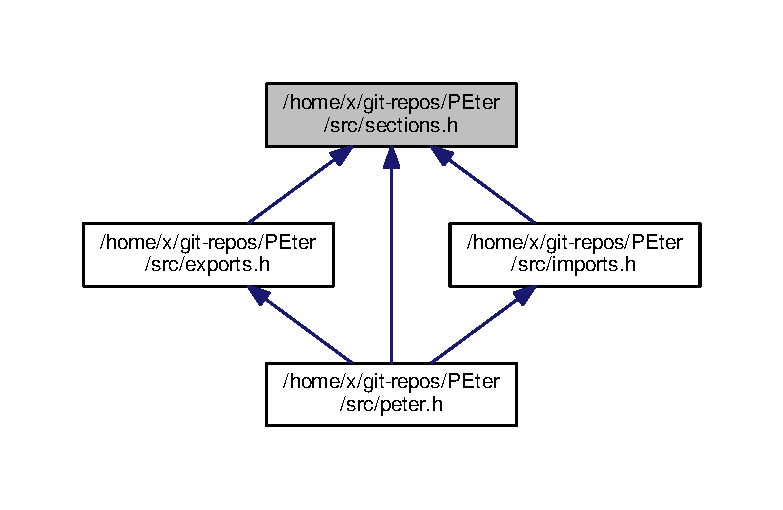
\includegraphics[width=350pt]{sections_8h__dep__incl}
\end{center}
\end{figure}
\subsection*{Functions}
\begin{DoxyCompactItemize}
\item 
I\+M\+A\+G\+E\+\_\+\+S\+E\+C\+T\+I\+O\+N\+\_\+\+H\+E\+A\+D\+ER $\ast$ \hyperlink{sections_8h_a1607507fea9b1d571bcd2b1dba7767ed}{sections\+\_\+by\+\_\+index\+\_\+get\+\_\+sh} (void $\ast$image, int index)
\begin{DoxyCompactList}\small\item\em returns a pointer on the I\+M\+A\+G\+E\+\_\+\+S\+E\+C\+T\+I\+O\+N\+\_\+\+H\+E\+A\+D\+ER at the indexed poisition. \end{DoxyCompactList}\item 
I\+M\+A\+G\+E\+\_\+\+S\+E\+C\+T\+I\+O\+N\+\_\+\+H\+E\+A\+D\+ER $\ast$ \hyperlink{sections_8h_a73bf53a38fec810d4d292c3a289b4d34}{sections\+\_\+by\+\_\+name\+\_\+get\+\_\+sh} (void $\ast$image, const char $\ast$name)
\begin{DoxyCompactList}\small\item\em like \hyperlink{sections_8h_a1607507fea9b1d571bcd2b1dba7767ed}{sections\+\_\+by\+\_\+index\+\_\+get\+\_\+sh()} but index is replaced by the section name. \end{DoxyCompactList}\item 
int \hyperlink{sections_8h_a1d9de14ada9284caacc29508c244d1a0}{sections\+\_\+by\+\_\+name\+\_\+get\+\_\+index} (void $\ast$image, const char $\ast$name)
\begin{DoxyCompactList}\small\item\em Tells you at which position the section header with the name xy lies. \end{DoxyCompactList}\item 
uint32\+\_\+t \hyperlink{sections_8h_acecc15a9fe93f6aff2414aa293930304}{sections\+\_\+by\+\_\+name\+\_\+get\+\_\+characteristics} (void $\ast$image, const char $\ast$name)
\begin{DoxyCompactList}\small\item\em returns the characteristics field of a section header. \end{DoxyCompactList}\item 
char $\ast$ \hyperlink{sections_8h_a5d187005583cbb3615b678fec1e6a89f}{sections\+\_\+by\+\_\+index\+\_\+get\+\_\+name} (void $\ast$image, int idx)
\begin{DoxyCompactList}\small\item\em returns the name of the section nr idx \end{DoxyCompactList}\item 
int \hyperlink{sections_8h_a4846d5524cb1771349480ba3fa53aa5b}{sections\+\_\+by\+\_\+name\+\_\+is\+\_\+writable} (void $\ast$image, const char $\ast$name)
\begin{DoxyCompactList}\small\item\em returns 1 if the section is writable and 0 if not \end{DoxyCompactList}\item 
int \hyperlink{sections_8h_a5bd5feff55b4788ddceb3eef54949883}{sections\+\_\+by\+\_\+name\+\_\+is\+\_\+readable} (void $\ast$image, const char $\ast$name)
\begin{DoxyCompactList}\small\item\em returns 1 if section is readable and 0 if not \end{DoxyCompactList}\item 
int \hyperlink{sections_8h_a65dbf84957c717cff8a45fb2a54bd45d}{sections\+\_\+by\+\_\+name\+\_\+is\+\_\+executable} (void $\ast$image, const char $\ast$name)
\begin{DoxyCompactList}\small\item\em returns 1 if the section is executable and 0 if not. \end{DoxyCompactList}\item 
void $\ast$ \hyperlink{sections_8h_a7a7e6c2a747698c2ebbcc8c3ce2dafcb}{sections\+\_\+by\+\_\+name\+\_\+get\+\_\+pointer\+\_\+to\+\_\+memory} (void $\ast$image, const char $\ast$name)
\begin{DoxyCompactList}\small\item\em returns a pointer on the first byte of a section \end{DoxyCompactList}\item 
uint32\+\_\+t \hyperlink{sections_8h_ae3615c254cdce0b7a85f39551da83f5a}{rva\+\_\+to\+\_\+raw} (char $\ast$image, uint32\+\_\+t rva)
\begin{DoxyCompactList}\small\item\em you give it a 32bit rva and it returns the raw offset \end{DoxyCompactList}\item 
void $\ast$ \hyperlink{sections_8h_aae919f2a09adf5893319fbf816e5c504}{rva\+\_\+to\+\_\+ptr} (void $\ast$image, uint32\+\_\+t rva)
\item 
uint32\+\_\+t \hyperlink{sections_8h_ae8714694bd5ece651dd403b3b0a20e6e}{raw\+\_\+to\+\_\+rva} (char $\ast$image, uint32\+\_\+t raw)
\begin{DoxyCompactList}\small\item\em returns a rva if you give it a raw offset \end{DoxyCompactList}\item 
\mbox{\Hypertarget{sections_8h_a6b9a4542a97e777e4a785802ba642d2e}\label{sections_8h_a6b9a4542a97e777e4a785802ba642d2e}} 
uint32\+\_\+t {\bfseries ptr\+\_\+to\+\_\+rva} (void $\ast$image, void $\ast$ptr)
\item 
void \hyperlink{sections_8h_a78d9de376d9fff273c7748f2cbebee19}{sections\+\_\+by\+\_\+name\+\_\+set\+\_\+writable} (void $\ast$image, const char $\ast$name)
\begin{DoxyCompactList}\small\item\em Sets the writable flag in the section header. \end{DoxyCompactList}\item 
void \hyperlink{sections_8h_ad4609b930147a7b9bfc486dd9fdb3657}{sections\+\_\+by\+\_\+name\+\_\+set\+\_\+readable} (void $\ast$image, const char $\ast$name)
\begin{DoxyCompactList}\small\item\em sets the readable flag in the section header \end{DoxyCompactList}\item 
void \hyperlink{sections_8h_ab04cc9185024a2a99770aa1f97253ff2}{sections\+\_\+by\+\_\+name\+\_\+set\+\_\+executable} (void $\ast$image, const char $\ast$name)
\begin{DoxyCompactList}\small\item\em sets the executable flag in the section header \end{DoxyCompactList}\item 
void \hyperlink{sections_8h_af3c1453de2d6655bf83c8373237cbf67}{sections\+\_\+by\+\_\+name\+\_\+set\+\_\+name} (void $\ast$image, const char $\ast$name, const char $\ast$replace)
\begin{DoxyCompactList}\small\item\em replaces the section name with a section name of your choise (8 byte max) \end{DoxyCompactList}\item 
void \hyperlink{sections_8h_a3059f46d8ebc5a2f66459d118a514a69}{sections\+\_\+by\+\_\+name\+\_\+set\+\_\+characteristics} (void $\ast$image, const char $\ast$name, uint32\+\_\+t characteristics)
\begin{DoxyCompactList}\small\item\em sets the characteristics field of a section header. \end{DoxyCompactList}\item 
void $\ast$ \hyperlink{sections_8h_ad4839ef873c682f604bd9f91c3354f8c}{sections\+\_\+add\+\_\+section} (void $\ast$image, int image\+Sz, void $\ast$space\+Ret\+Image, int space\+Sz, const char $\ast$name, uint32\+\_\+t size)
\begin{DoxyCompactList}\small\item\em Creates a new PE image from image. The new image will be written to space\+Space\+Ret\+Image is there is enough space. The new image will be like the old but with a section added to it. You can calculate the number of bytes you must allocate with\+: \hyperlink{sections_8h_a237b886e3fab53524e7d63d4064aa9dc}{sections\+\_\+get\+\_\+sizeof\+\_\+image\+\_\+after\+\_\+add\+\_\+section()}. The return value is a pointer on the first byte of the new section. \end{DoxyCompactList}\item 
uint32\+\_\+t \hyperlink{sections_8h_a237b886e3fab53524e7d63d4064aa9dc}{sections\+\_\+get\+\_\+sizeof\+\_\+image\+\_\+after\+\_\+add\+\_\+section} (void $\ast$old\+Image, uint32\+\_\+t old\+Sz, uint32\+\_\+t added\+Sz)
\begin{DoxyCompactList}\small\item\em calculates the size, the image will have after adding a section \end{DoxyCompactList}\item 
void $\ast$ \hyperlink{sections_8h_a2c89350109042cf56a310b23f8a2c999}{sections\+\_\+by\+\_\+name\+\_\+enlarge} (void $\ast$image, const char $\ast$name, char $\ast$bytes, uint32\+\_\+t bytes\+Len)
\begin{DoxyCompactList}\small\item\em enlarges a section and returns a pointer on the first byte of the new allocated space. If it fails it returns N\+U\+LL. \end{DoxyCompactList}\end{DoxyCompactItemize}


\subsection{Detailed Description}
This file contains functions for getting information concerning the section headers (e.\+g. \hyperlink{sections_8h_a4846d5524cb1771349480ba3fa53aa5b}{sections\+\_\+by\+\_\+name\+\_\+is\+\_\+writable()} informs you wether the writable flag in a section header is set). An other type of function changes the values within the section headers (set functions like \hyperlink{sections_8h_af3c1453de2d6655bf83c8373237cbf67}{sections\+\_\+by\+\_\+name\+\_\+set\+\_\+name()} ) or may even add a new one. The functions which convert e.\+g. pointers to rva values where placed in this header too, because they need information from the section headers to calculate their return values. 



\subsection{Function Documentation}
\mbox{\Hypertarget{sections_8h_ae8714694bd5ece651dd403b3b0a20e6e}\label{sections_8h_ae8714694bd5ece651dd403b3b0a20e6e}} 
\index{sections.\+h@{sections.\+h}!raw\+\_\+to\+\_\+rva@{raw\+\_\+to\+\_\+rva}}
\index{raw\+\_\+to\+\_\+rva@{raw\+\_\+to\+\_\+rva}!sections.\+h@{sections.\+h}}
\subsubsection{\texorpdfstring{raw\+\_\+to\+\_\+rva()}{raw\_to\_rva()}}
{\footnotesize\ttfamily uint32\+\_\+t raw\+\_\+to\+\_\+rva (\begin{DoxyParamCaption}\item[{char $\ast$}]{image,  }\item[{uint32\+\_\+t}]{raw }\end{DoxyParamCaption})}



returns a rva if you give it a raw offset 


\begin{DoxyParams}{Parameters}
{\em image} & \\
\hline
{\em raw} & \\
\hline
\end{DoxyParams}
\mbox{\Hypertarget{sections_8h_aae919f2a09adf5893319fbf816e5c504}\label{sections_8h_aae919f2a09adf5893319fbf816e5c504}} 
\index{sections.\+h@{sections.\+h}!rva\+\_\+to\+\_\+ptr@{rva\+\_\+to\+\_\+ptr}}
\index{rva\+\_\+to\+\_\+ptr@{rva\+\_\+to\+\_\+ptr}!sections.\+h@{sections.\+h}}
\subsubsection{\texorpdfstring{rva\+\_\+to\+\_\+ptr()}{rva\_to\_ptr()}}
{\footnotesize\ttfamily void$\ast$ rva\+\_\+to\+\_\+ptr (\begin{DoxyParamCaption}\item[{void $\ast$}]{image,  }\item[{uint32\+\_\+t}]{rva }\end{DoxyParamCaption})}


\begin{DoxyParams}{Parameters}
{\em image} & \\
\hline
{\em rva} & \\
\hline
\end{DoxyParams}
\mbox{\Hypertarget{sections_8h_ae3615c254cdce0b7a85f39551da83f5a}\label{sections_8h_ae3615c254cdce0b7a85f39551da83f5a}} 
\index{sections.\+h@{sections.\+h}!rva\+\_\+to\+\_\+raw@{rva\+\_\+to\+\_\+raw}}
\index{rva\+\_\+to\+\_\+raw@{rva\+\_\+to\+\_\+raw}!sections.\+h@{sections.\+h}}
\subsubsection{\texorpdfstring{rva\+\_\+to\+\_\+raw()}{rva\_to\_raw()}}
{\footnotesize\ttfamily uint32\+\_\+t rva\+\_\+to\+\_\+raw (\begin{DoxyParamCaption}\item[{char $\ast$}]{image,  }\item[{uint32\+\_\+t}]{rva }\end{DoxyParamCaption})}



you give it a 32bit rva and it returns the raw offset 


\begin{DoxyParams}{Parameters}
{\em image} & is the PE file. \\
\hline
{\em rva} & \\
\hline
\end{DoxyParams}
\mbox{\Hypertarget{sections_8h_ad4839ef873c682f604bd9f91c3354f8c}\label{sections_8h_ad4839ef873c682f604bd9f91c3354f8c}} 
\index{sections.\+h@{sections.\+h}!sections\+\_\+add\+\_\+section@{sections\+\_\+add\+\_\+section}}
\index{sections\+\_\+add\+\_\+section@{sections\+\_\+add\+\_\+section}!sections.\+h@{sections.\+h}}
\subsubsection{\texorpdfstring{sections\+\_\+add\+\_\+section()}{sections\_add\_section()}}
{\footnotesize\ttfamily void$\ast$ sections\+\_\+add\+\_\+section (\begin{DoxyParamCaption}\item[{void $\ast$}]{image,  }\item[{int}]{image\+Sz,  }\item[{void $\ast$}]{space\+Ret\+Image,  }\item[{int}]{space\+Sz,  }\item[{const char $\ast$}]{name,  }\item[{uint32\+\_\+t}]{size }\end{DoxyParamCaption})}



Creates a new PE image from image. The new image will be written to space\+Space\+Ret\+Image is there is enough space. The new image will be like the old but with a section added to it. You can calculate the number of bytes you must allocate with\+: \hyperlink{sections_8h_a237b886e3fab53524e7d63d4064aa9dc}{sections\+\_\+get\+\_\+sizeof\+\_\+image\+\_\+after\+\_\+add\+\_\+section()}. The return value is a pointer on the first byte of the new section. 


\begin{DoxyParams}{Parameters}
{\em image} & is the old pe image \\
\hline
{\em image\+Sz} & is the size of the old image in bytes \\
\hline
{\em space\+Ret\+Image} & should point on an allocated space in memory \\
\hline
{\em space\+Sz} & must contain the size in bytes of the memory space\+Ret\+Image is pointing to. \\
\hline
{\em name} & is the name of the new section (not longer than 8 bytes) \\
\hline
{\em size} & is how big you want the new section to be (in bytes) \\
\hline
\end{DoxyParams}
\mbox{\Hypertarget{sections_8h_a5d187005583cbb3615b678fec1e6a89f}\label{sections_8h_a5d187005583cbb3615b678fec1e6a89f}} 
\index{sections.\+h@{sections.\+h}!sections\+\_\+by\+\_\+index\+\_\+get\+\_\+name@{sections\+\_\+by\+\_\+index\+\_\+get\+\_\+name}}
\index{sections\+\_\+by\+\_\+index\+\_\+get\+\_\+name@{sections\+\_\+by\+\_\+index\+\_\+get\+\_\+name}!sections.\+h@{sections.\+h}}
\subsubsection{\texorpdfstring{sections\+\_\+by\+\_\+index\+\_\+get\+\_\+name()}{sections\_by\_index\_get\_name()}}
{\footnotesize\ttfamily char$\ast$ sections\+\_\+by\+\_\+index\+\_\+get\+\_\+name (\begin{DoxyParamCaption}\item[{void $\ast$}]{image,  }\item[{int}]{idx }\end{DoxyParamCaption})}



returns the name of the section nr idx 


\begin{DoxyParams}{Parameters}
{\em index} & is the PE file. \\
\hline
{\em idx} & is the section index (starts with 0) \\
\hline
\end{DoxyParams}
\mbox{\Hypertarget{sections_8h_a1607507fea9b1d571bcd2b1dba7767ed}\label{sections_8h_a1607507fea9b1d571bcd2b1dba7767ed}} 
\index{sections.\+h@{sections.\+h}!sections\+\_\+by\+\_\+index\+\_\+get\+\_\+sh@{sections\+\_\+by\+\_\+index\+\_\+get\+\_\+sh}}
\index{sections\+\_\+by\+\_\+index\+\_\+get\+\_\+sh@{sections\+\_\+by\+\_\+index\+\_\+get\+\_\+sh}!sections.\+h@{sections.\+h}}
\subsubsection{\texorpdfstring{sections\+\_\+by\+\_\+index\+\_\+get\+\_\+sh()}{sections\_by\_index\_get\_sh()}}
{\footnotesize\ttfamily I\+M\+A\+G\+E\+\_\+\+S\+E\+C\+T\+I\+O\+N\+\_\+\+H\+E\+A\+D\+ER$\ast$ sections\+\_\+by\+\_\+index\+\_\+get\+\_\+sh (\begin{DoxyParamCaption}\item[{void $\ast$}]{image,  }\item[{int}]{index }\end{DoxyParamCaption})}



returns a pointer on the I\+M\+A\+G\+E\+\_\+\+S\+E\+C\+T\+I\+O\+N\+\_\+\+H\+E\+A\+D\+ER at the indexed poisition. 


\begin{DoxyParams}{Parameters}
{\em image} & is a pointer on the PE file in memory. \\
\hline
{\em index} & starts with 0 and is 1 if you want the second section header. \\
\hline
\end{DoxyParams}
\mbox{\Hypertarget{sections_8h_a2c89350109042cf56a310b23f8a2c999}\label{sections_8h_a2c89350109042cf56a310b23f8a2c999}} 
\index{sections.\+h@{sections.\+h}!sections\+\_\+by\+\_\+name\+\_\+enlarge@{sections\+\_\+by\+\_\+name\+\_\+enlarge}}
\index{sections\+\_\+by\+\_\+name\+\_\+enlarge@{sections\+\_\+by\+\_\+name\+\_\+enlarge}!sections.\+h@{sections.\+h}}
\subsubsection{\texorpdfstring{sections\+\_\+by\+\_\+name\+\_\+enlarge()}{sections\_by\_name\_enlarge()}}
{\footnotesize\ttfamily void$\ast$ sections\+\_\+by\+\_\+name\+\_\+enlarge (\begin{DoxyParamCaption}\item[{void $\ast$}]{image,  }\item[{const char $\ast$}]{name,  }\item[{char $\ast$}]{bytes,  }\item[{uint32\+\_\+t}]{bytes\+Len }\end{DoxyParamCaption})}



enlarges a section and returns a pointer on the first byte of the new allocated space. If it fails it returns N\+U\+LL. 


\begin{DoxyParams}{Parameters}
{\em image} & is the PE image \\
\hline
{\em name} & is the name of the section you want to enlarge \\
\hline
{\em bytes} & are the bytes you want to add to the section. It can be N\+U\+LL. \\
\hline
{\em bytes\+Len} & is the size in bytes by which you want the section to be enlarged. \\
\hline
\end{DoxyParams}
\mbox{\Hypertarget{sections_8h_acecc15a9fe93f6aff2414aa293930304}\label{sections_8h_acecc15a9fe93f6aff2414aa293930304}} 
\index{sections.\+h@{sections.\+h}!sections\+\_\+by\+\_\+name\+\_\+get\+\_\+characteristics@{sections\+\_\+by\+\_\+name\+\_\+get\+\_\+characteristics}}
\index{sections\+\_\+by\+\_\+name\+\_\+get\+\_\+characteristics@{sections\+\_\+by\+\_\+name\+\_\+get\+\_\+characteristics}!sections.\+h@{sections.\+h}}
\subsubsection{\texorpdfstring{sections\+\_\+by\+\_\+name\+\_\+get\+\_\+characteristics()}{sections\_by\_name\_get\_characteristics()}}
{\footnotesize\ttfamily uint32\+\_\+t sections\+\_\+by\+\_\+name\+\_\+get\+\_\+characteristics (\begin{DoxyParamCaption}\item[{void $\ast$}]{image,  }\item[{const char $\ast$}]{name }\end{DoxyParamCaption})}



returns the characteristics field of a section header. 


\begin{DoxyParams}{Parameters}
{\em image} & is like always the PE file. \\
\hline
{\em name} & is the section name. \\
\hline
\end{DoxyParams}
\mbox{\Hypertarget{sections_8h_a1d9de14ada9284caacc29508c244d1a0}\label{sections_8h_a1d9de14ada9284caacc29508c244d1a0}} 
\index{sections.\+h@{sections.\+h}!sections\+\_\+by\+\_\+name\+\_\+get\+\_\+index@{sections\+\_\+by\+\_\+name\+\_\+get\+\_\+index}}
\index{sections\+\_\+by\+\_\+name\+\_\+get\+\_\+index@{sections\+\_\+by\+\_\+name\+\_\+get\+\_\+index}!sections.\+h@{sections.\+h}}
\subsubsection{\texorpdfstring{sections\+\_\+by\+\_\+name\+\_\+get\+\_\+index()}{sections\_by\_name\_get\_index()}}
{\footnotesize\ttfamily int sections\+\_\+by\+\_\+name\+\_\+get\+\_\+index (\begin{DoxyParamCaption}\item[{void $\ast$}]{image,  }\item[{const char $\ast$}]{name }\end{DoxyParamCaption})}



Tells you at which position the section header with the name xy lies. 


\begin{DoxyParams}{Parameters}
{\em image} & is the PE file. \\
\hline
{\em name} & is the name of the section (max 8 byte) \\
\hline
\end{DoxyParams}
\mbox{\Hypertarget{sections_8h_a7a7e6c2a747698c2ebbcc8c3ce2dafcb}\label{sections_8h_a7a7e6c2a747698c2ebbcc8c3ce2dafcb}} 
\index{sections.\+h@{sections.\+h}!sections\+\_\+by\+\_\+name\+\_\+get\+\_\+pointer\+\_\+to\+\_\+memory@{sections\+\_\+by\+\_\+name\+\_\+get\+\_\+pointer\+\_\+to\+\_\+memory}}
\index{sections\+\_\+by\+\_\+name\+\_\+get\+\_\+pointer\+\_\+to\+\_\+memory@{sections\+\_\+by\+\_\+name\+\_\+get\+\_\+pointer\+\_\+to\+\_\+memory}!sections.\+h@{sections.\+h}}
\subsubsection{\texorpdfstring{sections\+\_\+by\+\_\+name\+\_\+get\+\_\+pointer\+\_\+to\+\_\+memory()}{sections\_by\_name\_get\_pointer\_to\_memory()}}
{\footnotesize\ttfamily void$\ast$ sections\+\_\+by\+\_\+name\+\_\+get\+\_\+pointer\+\_\+to\+\_\+memory (\begin{DoxyParamCaption}\item[{void $\ast$}]{image,  }\item[{const char $\ast$}]{name }\end{DoxyParamCaption})}



returns a pointer on the first byte of a section 


\begin{DoxyParams}{Parameters}
{\em image} & is the PE file. \\
\hline
{\em name} & is the section name. \\
\hline
\end{DoxyParams}
\mbox{\Hypertarget{sections_8h_a73bf53a38fec810d4d292c3a289b4d34}\label{sections_8h_a73bf53a38fec810d4d292c3a289b4d34}} 
\index{sections.\+h@{sections.\+h}!sections\+\_\+by\+\_\+name\+\_\+get\+\_\+sh@{sections\+\_\+by\+\_\+name\+\_\+get\+\_\+sh}}
\index{sections\+\_\+by\+\_\+name\+\_\+get\+\_\+sh@{sections\+\_\+by\+\_\+name\+\_\+get\+\_\+sh}!sections.\+h@{sections.\+h}}
\subsubsection{\texorpdfstring{sections\+\_\+by\+\_\+name\+\_\+get\+\_\+sh()}{sections\_by\_name\_get\_sh()}}
{\footnotesize\ttfamily I\+M\+A\+G\+E\+\_\+\+S\+E\+C\+T\+I\+O\+N\+\_\+\+H\+E\+A\+D\+ER$\ast$ sections\+\_\+by\+\_\+name\+\_\+get\+\_\+sh (\begin{DoxyParamCaption}\item[{void $\ast$}]{image,  }\item[{const char $\ast$}]{name }\end{DoxyParamCaption})}



like \hyperlink{sections_8h_a1607507fea9b1d571bcd2b1dba7767ed}{sections\+\_\+by\+\_\+index\+\_\+get\+\_\+sh()} but index is replaced by the section name. 


\begin{DoxyParams}{Parameters}
{\em image} & is the PE file. \\
\hline
{\em name} & is a pointer on the section name. It should not exceed 8 bytes since the section names of PE files are not alowed to be longer than 8 bytes. \\
\hline
\end{DoxyParams}
\mbox{\Hypertarget{sections_8h_a65dbf84957c717cff8a45fb2a54bd45d}\label{sections_8h_a65dbf84957c717cff8a45fb2a54bd45d}} 
\index{sections.\+h@{sections.\+h}!sections\+\_\+by\+\_\+name\+\_\+is\+\_\+executable@{sections\+\_\+by\+\_\+name\+\_\+is\+\_\+executable}}
\index{sections\+\_\+by\+\_\+name\+\_\+is\+\_\+executable@{sections\+\_\+by\+\_\+name\+\_\+is\+\_\+executable}!sections.\+h@{sections.\+h}}
\subsubsection{\texorpdfstring{sections\+\_\+by\+\_\+name\+\_\+is\+\_\+executable()}{sections\_by\_name\_is\_executable()}}
{\footnotesize\ttfamily int sections\+\_\+by\+\_\+name\+\_\+is\+\_\+executable (\begin{DoxyParamCaption}\item[{void $\ast$}]{image,  }\item[{const char $\ast$}]{name }\end{DoxyParamCaption})}



returns 1 if the section is executable and 0 if not. 


\begin{DoxyParams}{Parameters}
{\em image} & is the PE file. \\
\hline
{\em name} & is the section name. \\
\hline
\end{DoxyParams}
\mbox{\Hypertarget{sections_8h_a5bd5feff55b4788ddceb3eef54949883}\label{sections_8h_a5bd5feff55b4788ddceb3eef54949883}} 
\index{sections.\+h@{sections.\+h}!sections\+\_\+by\+\_\+name\+\_\+is\+\_\+readable@{sections\+\_\+by\+\_\+name\+\_\+is\+\_\+readable}}
\index{sections\+\_\+by\+\_\+name\+\_\+is\+\_\+readable@{sections\+\_\+by\+\_\+name\+\_\+is\+\_\+readable}!sections.\+h@{sections.\+h}}
\subsubsection{\texorpdfstring{sections\+\_\+by\+\_\+name\+\_\+is\+\_\+readable()}{sections\_by\_name\_is\_readable()}}
{\footnotesize\ttfamily int sections\+\_\+by\+\_\+name\+\_\+is\+\_\+readable (\begin{DoxyParamCaption}\item[{void $\ast$}]{image,  }\item[{const char $\ast$}]{name }\end{DoxyParamCaption})}



returns 1 if section is readable and 0 if not 


\begin{DoxyParams}{Parameters}
{\em image} & is the PE file. \\
\hline
{\em name} & is the section name. \\
\hline
\end{DoxyParams}
\mbox{\Hypertarget{sections_8h_a4846d5524cb1771349480ba3fa53aa5b}\label{sections_8h_a4846d5524cb1771349480ba3fa53aa5b}} 
\index{sections.\+h@{sections.\+h}!sections\+\_\+by\+\_\+name\+\_\+is\+\_\+writable@{sections\+\_\+by\+\_\+name\+\_\+is\+\_\+writable}}
\index{sections\+\_\+by\+\_\+name\+\_\+is\+\_\+writable@{sections\+\_\+by\+\_\+name\+\_\+is\+\_\+writable}!sections.\+h@{sections.\+h}}
\subsubsection{\texorpdfstring{sections\+\_\+by\+\_\+name\+\_\+is\+\_\+writable()}{sections\_by\_name\_is\_writable()}}
{\footnotesize\ttfamily int sections\+\_\+by\+\_\+name\+\_\+is\+\_\+writable (\begin{DoxyParamCaption}\item[{void $\ast$}]{image,  }\item[{const char $\ast$}]{name }\end{DoxyParamCaption})}



returns 1 if the section is writable and 0 if not 


\begin{DoxyParams}{Parameters}
{\em image} & is the PE file. \\
\hline
{\em name} & is the section name \\
\hline
\end{DoxyParams}
\mbox{\Hypertarget{sections_8h_a3059f46d8ebc5a2f66459d118a514a69}\label{sections_8h_a3059f46d8ebc5a2f66459d118a514a69}} 
\index{sections.\+h@{sections.\+h}!sections\+\_\+by\+\_\+name\+\_\+set\+\_\+characteristics@{sections\+\_\+by\+\_\+name\+\_\+set\+\_\+characteristics}}
\index{sections\+\_\+by\+\_\+name\+\_\+set\+\_\+characteristics@{sections\+\_\+by\+\_\+name\+\_\+set\+\_\+characteristics}!sections.\+h@{sections.\+h}}
\subsubsection{\texorpdfstring{sections\+\_\+by\+\_\+name\+\_\+set\+\_\+characteristics()}{sections\_by\_name\_set\_characteristics()}}
{\footnotesize\ttfamily void sections\+\_\+by\+\_\+name\+\_\+set\+\_\+characteristics (\begin{DoxyParamCaption}\item[{void $\ast$}]{image,  }\item[{const char $\ast$}]{name,  }\item[{uint32\+\_\+t}]{characteristics }\end{DoxyParamCaption})}



sets the characteristics field of a section header. 


\begin{DoxyParams}{Parameters}
{\em image} & is the PE file. \\
\hline
{\em name} & is the name of the section \\
\hline
{\em characteristics} & is the value the characteristics filed should be changed to. \\
\hline
\end{DoxyParams}
\mbox{\Hypertarget{sections_8h_ab04cc9185024a2a99770aa1f97253ff2}\label{sections_8h_ab04cc9185024a2a99770aa1f97253ff2}} 
\index{sections.\+h@{sections.\+h}!sections\+\_\+by\+\_\+name\+\_\+set\+\_\+executable@{sections\+\_\+by\+\_\+name\+\_\+set\+\_\+executable}}
\index{sections\+\_\+by\+\_\+name\+\_\+set\+\_\+executable@{sections\+\_\+by\+\_\+name\+\_\+set\+\_\+executable}!sections.\+h@{sections.\+h}}
\subsubsection{\texorpdfstring{sections\+\_\+by\+\_\+name\+\_\+set\+\_\+executable()}{sections\_by\_name\_set\_executable()}}
{\footnotesize\ttfamily void sections\+\_\+by\+\_\+name\+\_\+set\+\_\+executable (\begin{DoxyParamCaption}\item[{void $\ast$}]{image,  }\item[{const char $\ast$}]{name }\end{DoxyParamCaption})}



sets the executable flag in the section header 


\begin{DoxyParams}{Parameters}
{\em image} & \\
\hline
{\em name} & \\
\hline
\end{DoxyParams}
\mbox{\Hypertarget{sections_8h_af3c1453de2d6655bf83c8373237cbf67}\label{sections_8h_af3c1453de2d6655bf83c8373237cbf67}} 
\index{sections.\+h@{sections.\+h}!sections\+\_\+by\+\_\+name\+\_\+set\+\_\+name@{sections\+\_\+by\+\_\+name\+\_\+set\+\_\+name}}
\index{sections\+\_\+by\+\_\+name\+\_\+set\+\_\+name@{sections\+\_\+by\+\_\+name\+\_\+set\+\_\+name}!sections.\+h@{sections.\+h}}
\subsubsection{\texorpdfstring{sections\+\_\+by\+\_\+name\+\_\+set\+\_\+name()}{sections\_by\_name\_set\_name()}}
{\footnotesize\ttfamily void sections\+\_\+by\+\_\+name\+\_\+set\+\_\+name (\begin{DoxyParamCaption}\item[{void $\ast$}]{image,  }\item[{const char $\ast$}]{name,  }\item[{const char $\ast$}]{replace }\end{DoxyParamCaption})}



replaces the section name with a section name of your choise (8 byte max) 


\begin{DoxyParams}{Parameters}
{\em image} & is the PE file \\
\hline
{\em name} & is the section name you want to replace \\
\hline
{\em replace} & is the new section name \\
\hline
\end{DoxyParams}
\mbox{\Hypertarget{sections_8h_ad4609b930147a7b9bfc486dd9fdb3657}\label{sections_8h_ad4609b930147a7b9bfc486dd9fdb3657}} 
\index{sections.\+h@{sections.\+h}!sections\+\_\+by\+\_\+name\+\_\+set\+\_\+readable@{sections\+\_\+by\+\_\+name\+\_\+set\+\_\+readable}}
\index{sections\+\_\+by\+\_\+name\+\_\+set\+\_\+readable@{sections\+\_\+by\+\_\+name\+\_\+set\+\_\+readable}!sections.\+h@{sections.\+h}}
\subsubsection{\texorpdfstring{sections\+\_\+by\+\_\+name\+\_\+set\+\_\+readable()}{sections\_by\_name\_set\_readable()}}
{\footnotesize\ttfamily void sections\+\_\+by\+\_\+name\+\_\+set\+\_\+readable (\begin{DoxyParamCaption}\item[{void $\ast$}]{image,  }\item[{const char $\ast$}]{name }\end{DoxyParamCaption})}



sets the readable flag in the section header 


\begin{DoxyParams}{Parameters}
{\em image} & \\
\hline
{\em name} & \\
\hline
\end{DoxyParams}
\mbox{\Hypertarget{sections_8h_a78d9de376d9fff273c7748f2cbebee19}\label{sections_8h_a78d9de376d9fff273c7748f2cbebee19}} 
\index{sections.\+h@{sections.\+h}!sections\+\_\+by\+\_\+name\+\_\+set\+\_\+writable@{sections\+\_\+by\+\_\+name\+\_\+set\+\_\+writable}}
\index{sections\+\_\+by\+\_\+name\+\_\+set\+\_\+writable@{sections\+\_\+by\+\_\+name\+\_\+set\+\_\+writable}!sections.\+h@{sections.\+h}}
\subsubsection{\texorpdfstring{sections\+\_\+by\+\_\+name\+\_\+set\+\_\+writable()}{sections\_by\_name\_set\_writable()}}
{\footnotesize\ttfamily void sections\+\_\+by\+\_\+name\+\_\+set\+\_\+writable (\begin{DoxyParamCaption}\item[{void $\ast$}]{image,  }\item[{const char $\ast$}]{name }\end{DoxyParamCaption})}



Sets the writable flag in the section header. 


\begin{DoxyParams}{Parameters}
{\em image} & is the PE image \\
\hline
{\em name} & is the section name \\
\hline
\end{DoxyParams}
\mbox{\Hypertarget{sections_8h_a237b886e3fab53524e7d63d4064aa9dc}\label{sections_8h_a237b886e3fab53524e7d63d4064aa9dc}} 
\index{sections.\+h@{sections.\+h}!sections\+\_\+get\+\_\+sizeof\+\_\+image\+\_\+after\+\_\+add\+\_\+section@{sections\+\_\+get\+\_\+sizeof\+\_\+image\+\_\+after\+\_\+add\+\_\+section}}
\index{sections\+\_\+get\+\_\+sizeof\+\_\+image\+\_\+after\+\_\+add\+\_\+section@{sections\+\_\+get\+\_\+sizeof\+\_\+image\+\_\+after\+\_\+add\+\_\+section}!sections.\+h@{sections.\+h}}
\subsubsection{\texorpdfstring{sections\+\_\+get\+\_\+sizeof\+\_\+image\+\_\+after\+\_\+add\+\_\+section()}{sections\_get\_sizeof\_image\_after\_add\_section()}}
{\footnotesize\ttfamily uint32\+\_\+t sections\+\_\+get\+\_\+sizeof\+\_\+image\+\_\+after\+\_\+add\+\_\+section (\begin{DoxyParamCaption}\item[{void $\ast$}]{old\+Image,  }\item[{uint32\+\_\+t}]{old\+Sz,  }\item[{uint32\+\_\+t}]{added\+Sz }\end{DoxyParamCaption})}



calculates the size, the image will have after adding a section 


\begin{DoxyParams}{Parameters}
{\em old\+Image} & is the PE image before adding a section \\
\hline
{\em old\+Sz} & is the size of the image, old\+Image is pointing to \\
\hline
{\em added\+Sz} & is the size of the section you want to add. \\
\hline
\end{DoxyParams}

%--- End generated contents ---

% Index
\backmatter
\newpage
\phantomsection
\clearemptydoublepage
\addcontentsline{toc}{chapter}{Index}
\printindex

\end{document}
